\newif\ifshowsolutions
\showsolutionstrue
\documentclass{article}
\usepackage{listings}
\usepackage{amsmath}
\usepackage{subfig}
\usepackage{amsthm}
\usepackage{amsmath}
\usepackage{amssymb}
\usepackage{graphicx}
\usepackage{mdwlist}
\usepackage{geometry}
\usepackage{titlesec}
\usepackage{palatino}
\usepackage{mathrsfs}
\usepackage{fancyhdr}
\usepackage{paralist}
\usepackage{todonotes}
\usepackage{tikz}
\usepackage{float} % Place figures where you ACTUALLY want it
\usepackage{comment} % A hack to toggle sections
\usepackage{ifthen}
\usepackage{mdframed}
\usepackage{verbatim}
\usepackage{listings}
\usepackage{bbm}
\usepackage{upquote} % Prevents backticks replacing single-quotes in verbatim
\usepackage[strings]{underscore}
\usepackage[colorlinks=true]{hyperref}
\usetikzlibrary{positioning,shapes,backgrounds}

\geometry{margin=1in}
\geometry{headheight=2in}
\geometry{top=2in}

\setlength{\marginparwidth}{2.15cm}
\setlength{\parindent}{0em}
\setlength{\parskip}{0.6\baselineskip}

\rhead{}
\lhead{}

% Spacing settings.
\titlespacing\section{0pt}{12pt plus 2pt minus 2pt}{0pt plus 2pt minus 2pt}
\titlespacing\subsection{0pt}{12pt plus 4pt minus 2pt}{0pt plus 2pt minus 2pt}
\titlespacing\subsubsection{0pt}{12pt plus 4pt minus 2pt}{0pt plus 2pt minus 2pt}
\renewcommand{\baselinestretch}{1.15}

% Shortcuts for commonly used operators.
\newcommand{\E}{\mathbb{E}}
\newcommand{\Var}{\operatorname{Var}}
\newcommand{\Cov}{\operatorname{Cov}}
\newcommand{\Bias}{\operatorname{Bias}}
\DeclareMathOperator{\argmin}{arg\,min}
\DeclareMathOperator{\argmax}{arg\,max}

% Do not number subsections and below.
\setcounter{secnumdepth}{1}

% Custom format subsection.
\titleformat*{\subsection}{\large\bfseries}

% Set up the problem environment.
\newcounter{problem}[section]
\newenvironment{problem}[1][]
  {\begingroup
    \setlength{\parskip}{0em}
    \refstepcounter{problem}\par\addvspace{1em}\textbf{Problem~\Alph{problem}\!
    \ifthenelse{\equal{#1}{}}{}{ [#1 points]}:}
  \endgroup}

% Set up the subproblem environment.
\newcounter{subproblem}[problem]
\newenvironment{subproblem}[1][]
  {\begingroup
    \setlength{\parskip}{0em}
    \refstepcounter{subproblem}\par\medskip\textbf{\roman{subproblem}.\!
    \ifthenelse{\equal{#1}{}}{}{ [#1 points]:}}
  \endgroup}

% Set up the teachers and materials commands.
\newcommand\teachers[1]
  {\begingroup
    \setlength{\parskip}{0em}
    \vspace{0.3em} \textit{\hspace*{2em} TAs responsible: #1} \par
  \endgroup}
\newcommand\materials[1]
  {\begingroup
    \setlength{\parskip}{0em}
    \textit{\hspace*{2em} Relevant materials: #1} \par \vspace{1em}
  \endgroup}

% Set up the hint environment.
\newenvironment{hint}[1][]
  {\begin{em}\textbf{Hint: }}
  {\end{em}}

% Set up the solution environment.
\ifshowsolutions
  \newenvironment{solution}[1][]
    {\par\medskip \begin{mdframed}\textbf{Solution~\Alph{problem}#1:} \begin{em}}
    {\end{em}\medskip\end{mdframed}\medskip}
  \newenvironment{subsolution}[1][]
    {\par\medskip \begin{mdframed}\textbf{Solution~\Alph{problem}#1.\roman{subproblem}:} \begin{em}}
    {\end{em}\medskip\end{mdframed}\medskip}
\else
  \excludecomment{solution}
  \excludecomment{subsolution}
\fi

\usepackage{array}
\newcolumntype{C}[1]{>{\centering\arraybackslash}p{#1}}

\usepackage{bbm}

%%%%%%%%%%%%%%%%%%%%%%%%%%%%%%
% HEADER
%%%%%%%%%%%%%%%%%%%%%%%%%%%%%%

\chead{
  {\vbox{
      \vspace{2mm}
      \large
      CS/CNS/EE 155 \hfill
      Philip Carr \hfill \\[1pt]
      Set 3\hfill \text{ }\\
      10 late hours were used for this set. \hfill
      %January $24^\text{th}$, 2019 \\
      January $30^\text{th}$, 2019 \\
    }
  }
}

\begin{document}
\pagestyle{fancy}


%%%%%%%%%%%%%%%%%%%%%%%%%%%%%%
% PROBLEM 1
%%%%%%%%%%%%%%%%%%%%%%%%%%%%%%

\newpage
\section{Decision Trees [30 Points]}
\materials{Lecture 5}

\problem[7] Consider the following data, where given information about some food you must
predict whether it is healthy:
\noindent
\begin{table}[H]
\centering
%\begin{tabular}{| C{0.5cm} | C{2cm} |}
\begin{tabular}{c | c c c | c}
\hline
No. & Package Type & Unit Price $>$ \$5 & Contains $>$ 5 grams of fat & Healthy? \\ \hline
1 & Canned & Yes & Yes & No \\
2 & Bagged & Yes & No & Yes \\
3 & Bagged & No & Yes & Yes \\
4 & Canned & No & No & Yes \\ \hline
\end{tabular}
\end{table}
\noindent
Train a decision tree by hand using top-down greedy induction. Use \textit{entropy} (with natural log) as the impurity measure. Since the data can be classified without error, the stopping criterion will be no impurity in the leaves.\\
\\
Submit a drawing of your tree showing the impurity reduction yielded by each split (including root) in your decision tree.
\begin{solution}\normalfont{
\noindent
\begin{figure}[H]
\centering
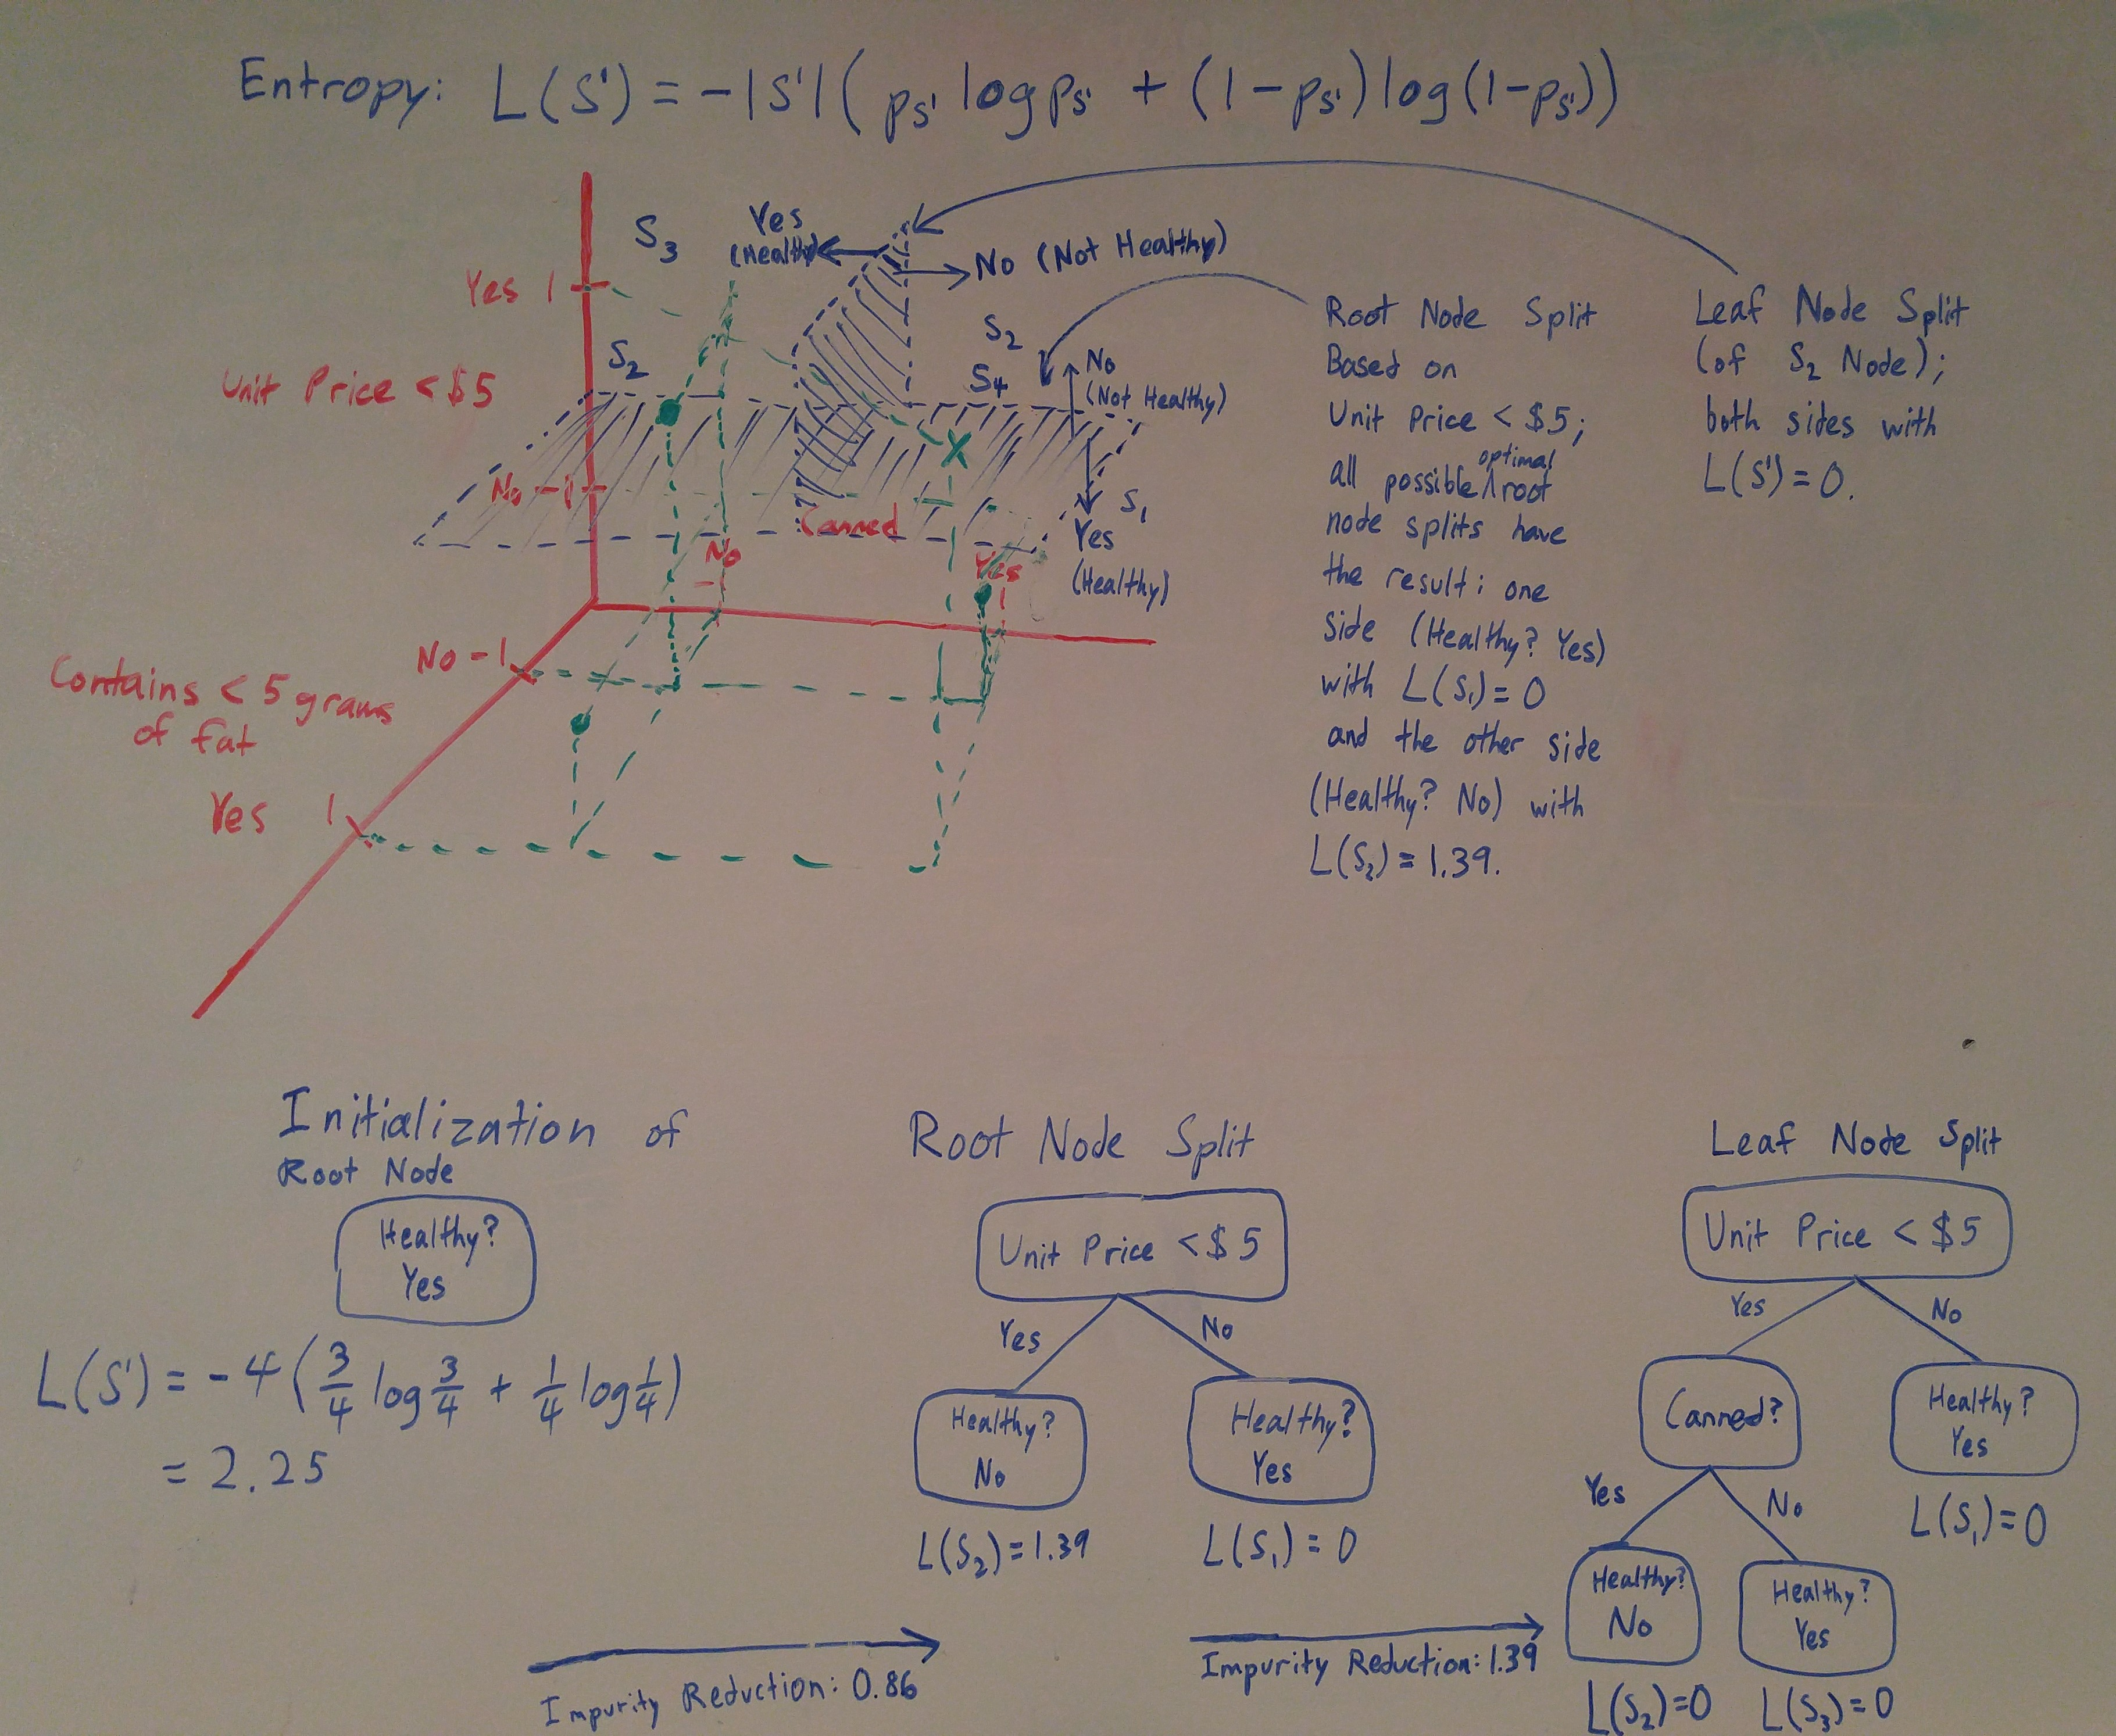
\includegraphics[scale=0.07]{1a_drawing.jpg}
\end{figure}
\noindent
Along the bottom of the image above is the decision tree as would make successive splits in the root and leaf nodes using top-down greedy induction, along with the impurity reduction yielded by each split (including the root) of the decision tree. The decision tree at the bottom right corner of the image is the completed decision tree with 0 impurity (all data classified without error). The question ``Canned?" refers to the feature Package Type, with yes and no responses to ``Canned" refering to Canned and Bagged respectively. All impurity measures shown in the image were calculated using entropy (with natural log).\\
\\
In the top left side of the image is a plot of the data points in the 3D feature space, where the dot points represent healthy food items, and where the x point represents the unhealthy food item. The decision tree in this plot is represented by its separating planes indicating the node boundaries of the decision tree.
}\end{solution}


\newpage
\problem[4] Compared to a linear classifier, is a decision tree always preferred for classification
problems? If not, draw a simple 2-D dataset that can be perfectly classified by a simple linear classifier but which requires an overly complex decision tree to perfectly classify.
\begin{solution}\normalfont{
Compared to a linear classifier, a decision tree is not always preferred for classification problems. One reason why this results is because decision trees only separate data points by boundaries parallel to some axis, but data points can end up being most easily separable along off-axis boundaries.\\
\\
Below is a drawing of a simple 2-D dataset that can be perfectly classified by a simple linear classifier but which requires an overly complex decision tree to perfectly classify (both the region with triangle points and the region with square points are split into two separate regions by the decision tree, while the linear classifier simply divides the points into their correct regions without an overly complicated model of the separated regions):
\noindent
\begin{figure}[H]
\centering
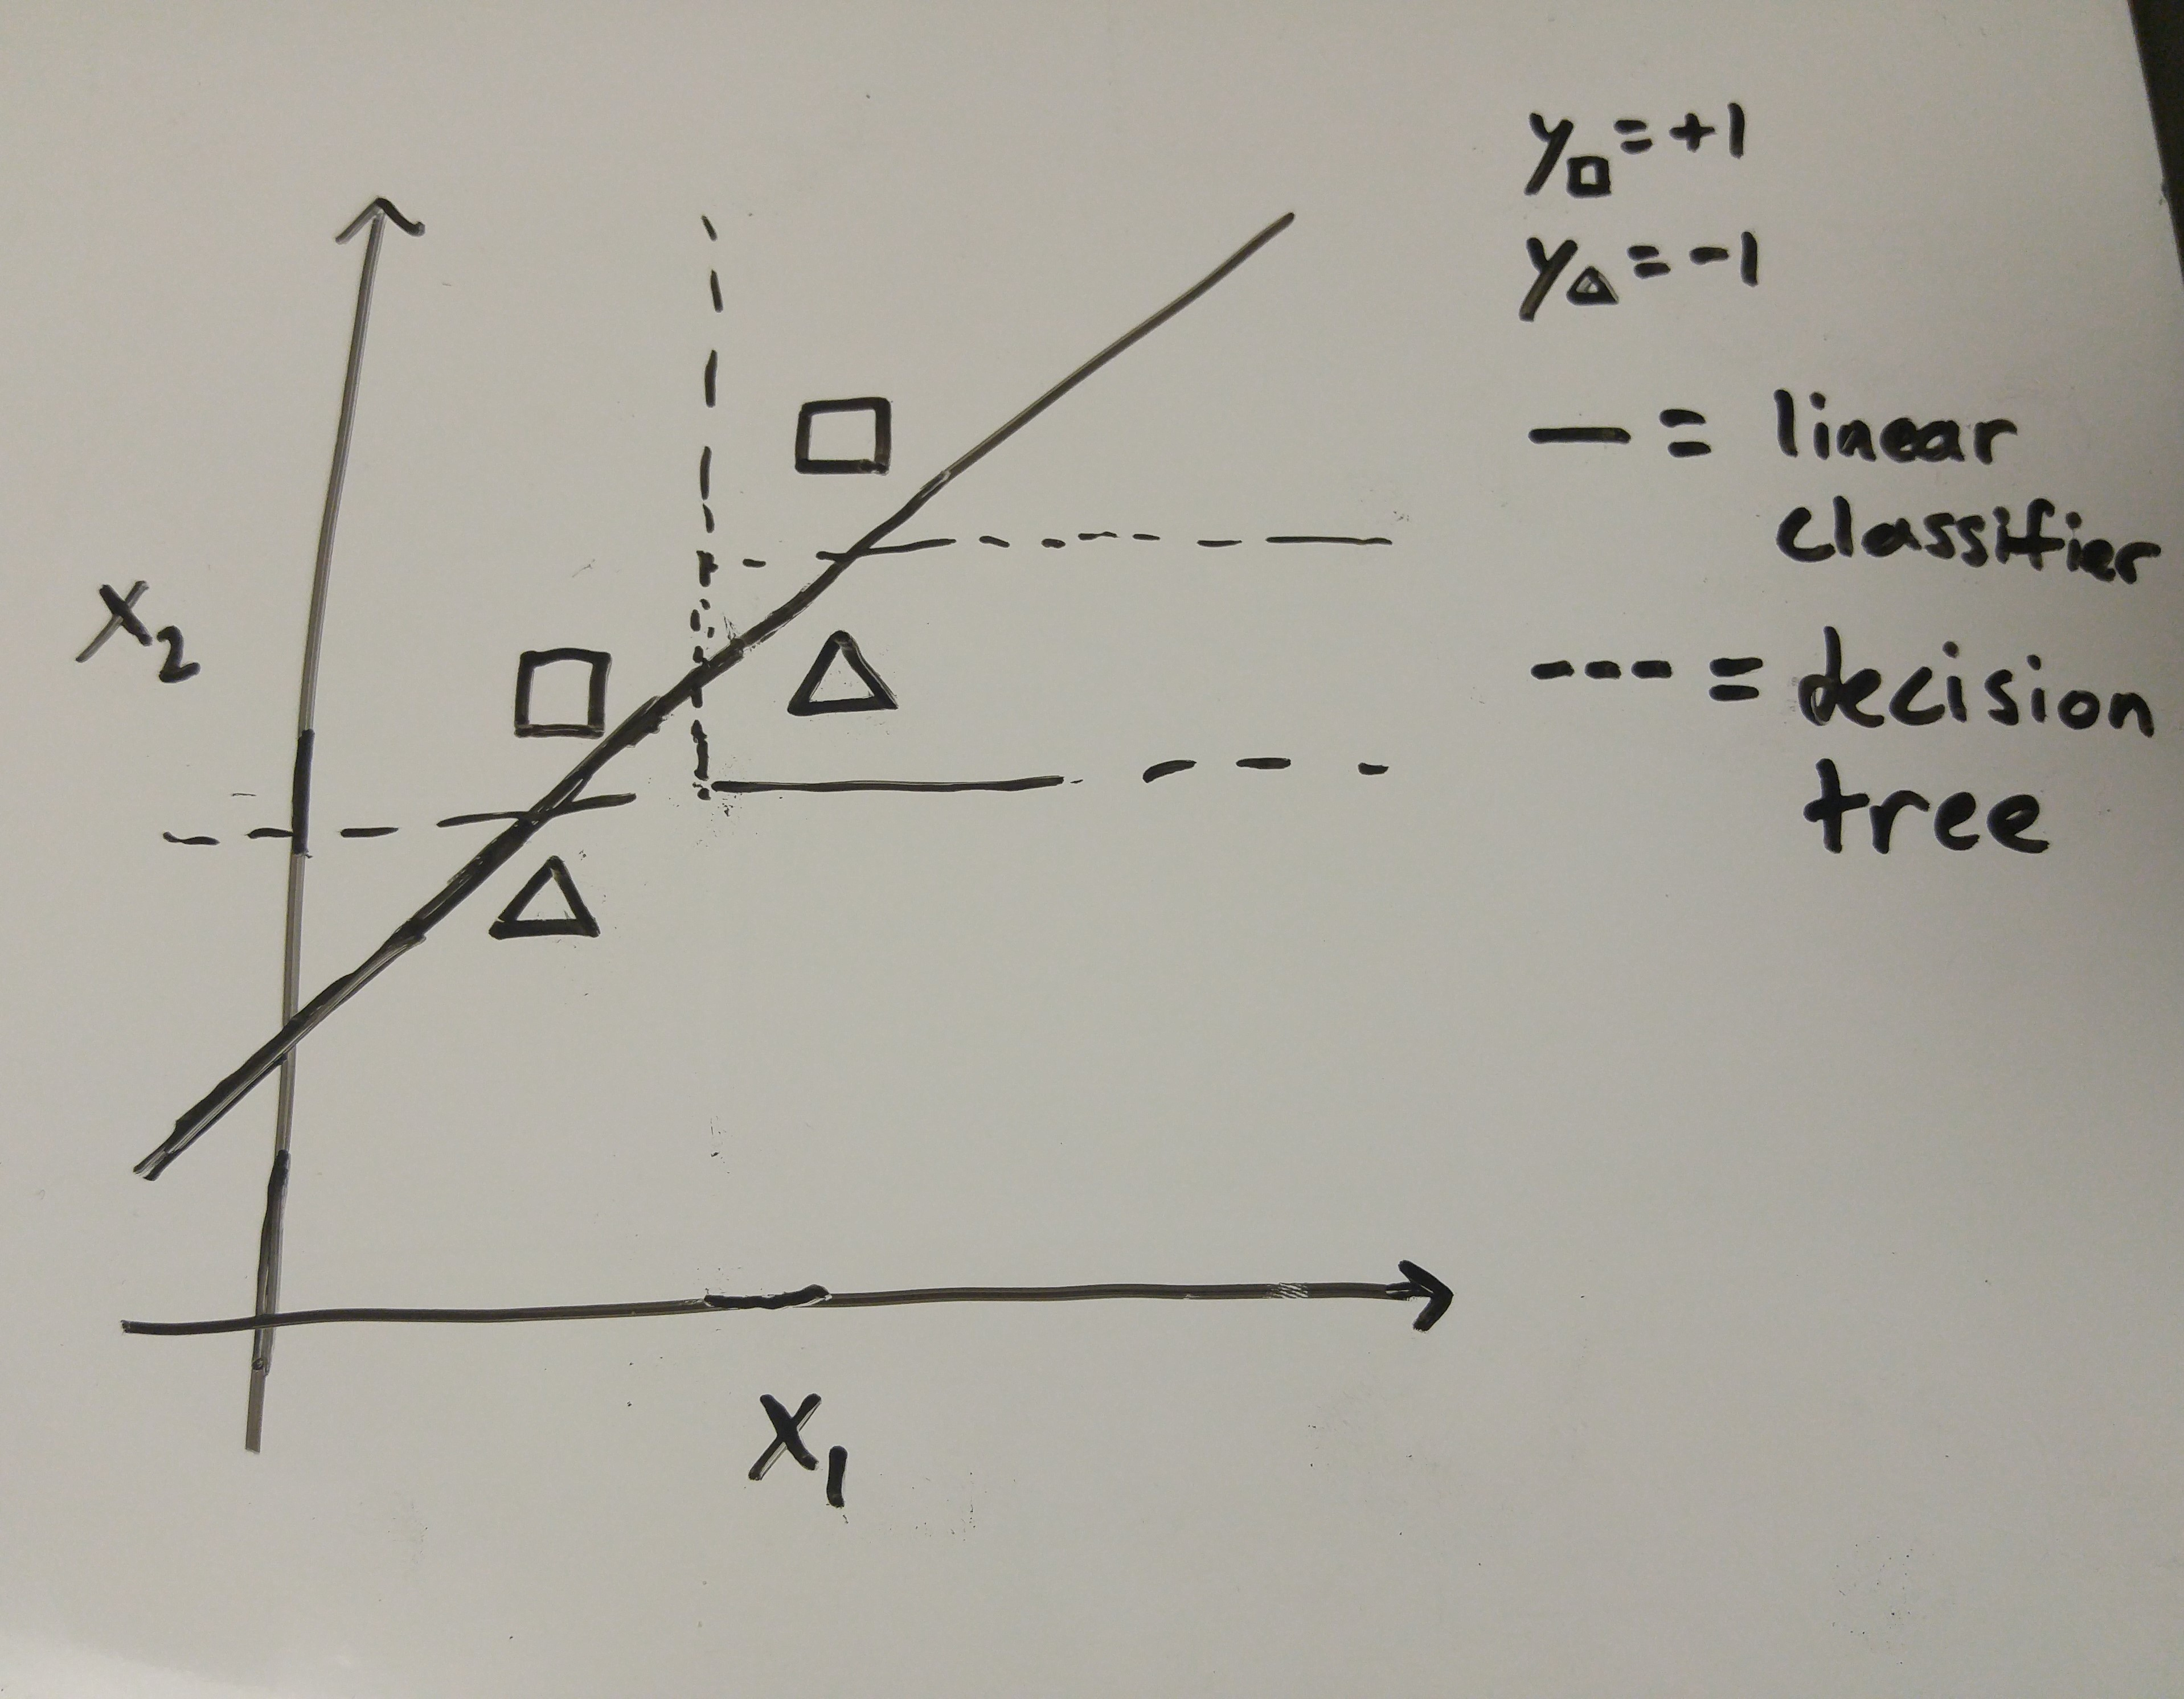
\includegraphics[scale=0.07]{1b_drawing.jpg}
\end{figure}
\noindent
}\end{solution}
\newpage


\problem[15] Consider the following 2D data set:
\noindent
\begin{figure}[H]
\centering
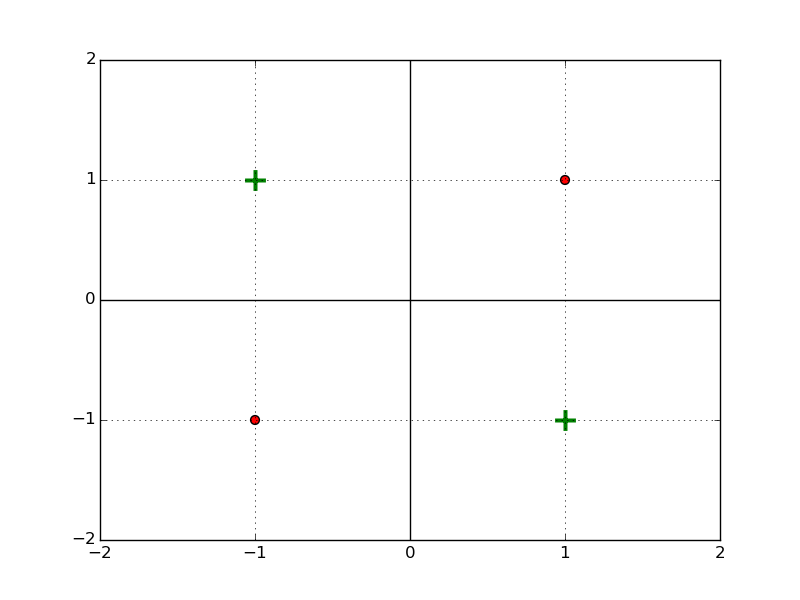
\includegraphics[scale=0.5]{1c_plot.png}
\end{figure}
\noindent
\subproblem[5] Suppose we train a decision tree on this dataset using top-down greedy induction, with the Gini index as the impurity measure. We define our stopping condition to be if no split of a node results in any reduction in impurity. Submit a drawing of the resulting tree. What is its classification error ((number of misclassified points) / (number of total points))?
\begin{subsolution}\normalfont{
\noindent
\begin{figure}[H]
\centering
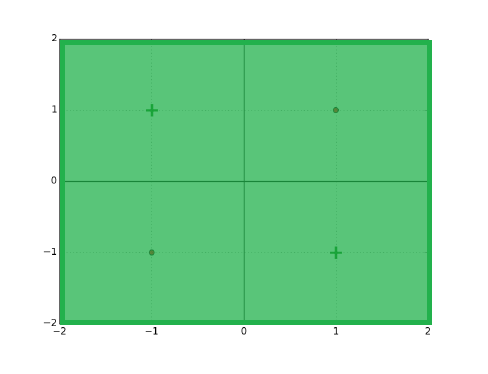
\includegraphics[scale=0.8]{1ci_plot.png}
\end{figure}
\noindent
At the initialization of the root node, all points in the dataset are classified as the majority class. In this dataset, both the green and red points are evenly represented, so without loss of generality, the root node was set to classify all points as green points (as indicated by the green shading over the entire space). This decision tree has a Gini index of $L(S') = \vert S' \vert (1 - p_{S'}^2 - (1 - p_{S'})^2) = (4)(1 - (\frac{1}{2})^2 - (1 - (\frac{1}{2})^2)) = 2$. Since every possible split of the root node results in the same Gini index of $L(S') = 2$, the root node is not split and the decision tree creation is stopped a the state shown above in the drawing.
}\end{subsolution}
\newpage


\subproblem[5] Submit a drawing of a two-level decision tree that classifies the above dataset with zero classification error. (You don’t need to use any particular training algorithm to produce the tree.)\\
\\
Is there any impurity measure (i.e. any function that maps the data points under a particular node in a tree to a real number) that would have led top-down greedy induction with the same stopping condition to produce the tree you drew? If so, give an example of one, and briefly describe its pros and cons as an impurity measure for training decision trees in general (on arbitrary datasets).
\begin{subsolution}\normalfont{
\noindent
\begin{figure}[H]
\centering
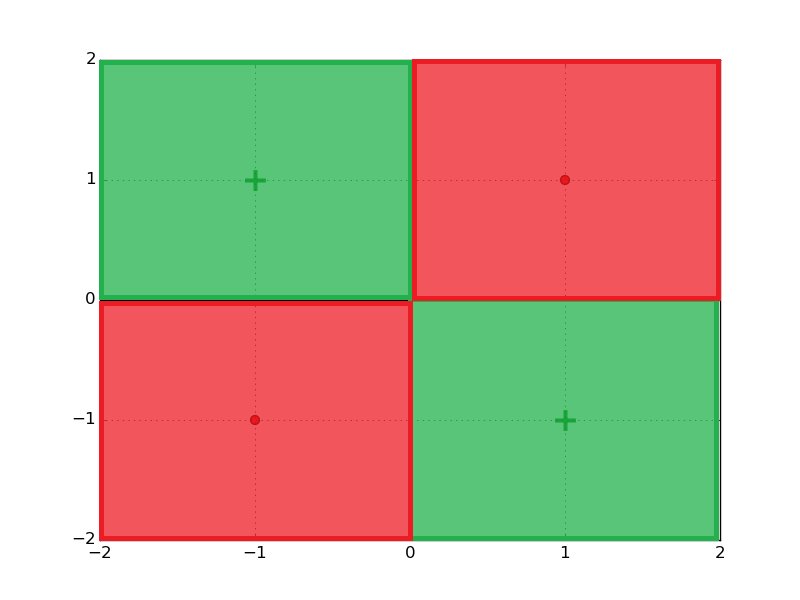
\includegraphics[scale=0.5]{1cii_plot.png}
\end{figure}
\noindent
Bernoulli measure $L(S') = \vert S' \vert - 1$
}\end{subsolution}
\newpage


\subproblem[5] Suppose there are 100 data points in some 2-D dataset. What is the largest number of unique thresholds (i.e., internal nodes) you might need in order to achieve zero classification training error (on the training set)? Please justify your answer.
\begin{subsolution}\normalfont{
\noindent
\begin{figure}[H]
\centering
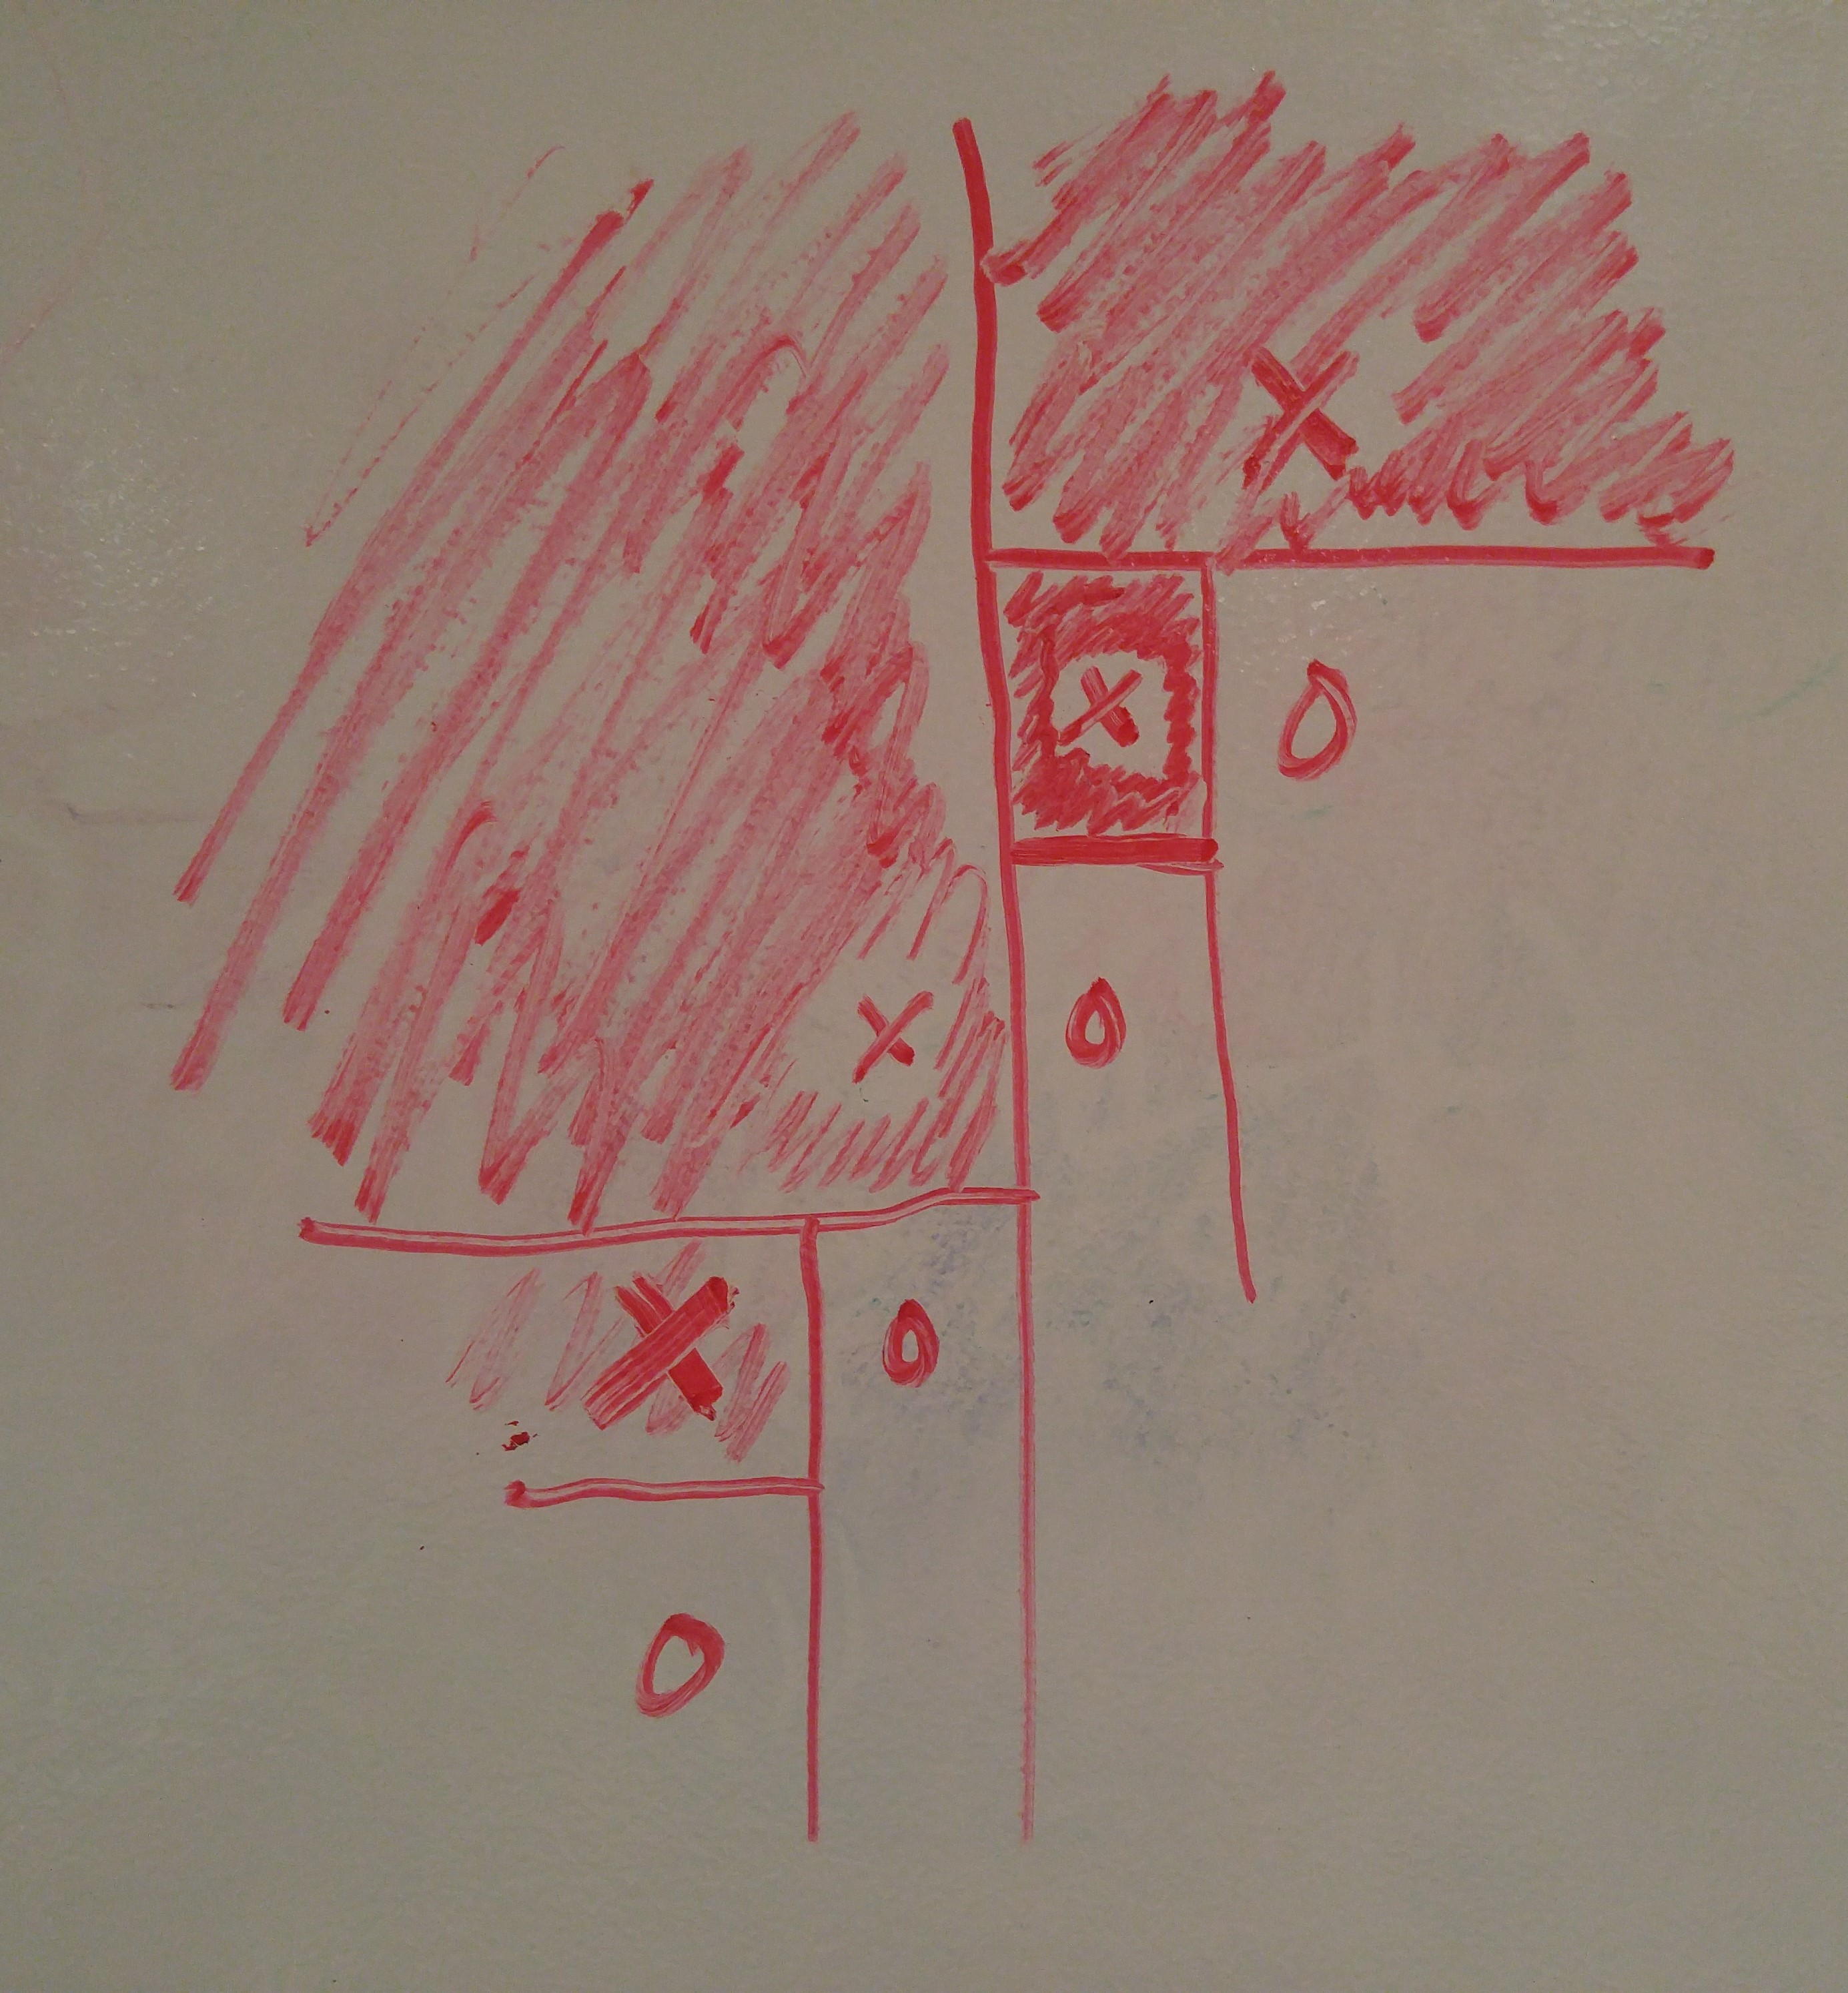
\includegraphics[scale=0.07]{1ciii_drawing.jpg}
\end{figure}
\noindent
As shown in the above example, data points arranged in this diagonal pattern will result in the decision tree having to make (a maximum of) as many unique thresholds as there are data points for the decision tree to achieve perfect classification training error (on the training set). Therefore, for 100 data points in some 2-D dataset, the largest number of unique thresholds needed to achieve zero classification training error (on the training set).
}\end{subsolution}
\newpage



\problem[4] Suppose in top-down greedy induction we want to split a leaf node that contains
N data points composed of D continuous features. What is the worst-case complexity (big-O in terms of N and D) of the number of possible splits we must consider in order to find the one that most reduces impurity? Please justify your answer.\\
\\
Note: Recall that at each node-splitting step in training a DT, you must consider all possible splits that you can make. While there are an infinite number of possible decision boundaries since we are using continuous features, there are not an infinite number of boundaries that result in unique child sets (which is what we mean by “split”).
\begin{solution}\normalfont{
At each node-splitting step in training a DT, all possible splits that can be made all must be considered. Because of this, the number of possible unique splits (where a unique split is distinct from other splits in terms of which data points are located in one side of the decision tree split or the other) is linearly proportional to the number of data points $N$, so this operation's complexity is $O(N)$. Since there are $D$ dimesions of the dataset, all possible splits in all possible dimensions must also be made. Thus, this operation's complexity is linearly proportional to $D$, so this operation's complexity is $O(D)$. Combining the two operations, since the decision tree model iterates through all possible splits of the $N$ data points for each dimension $D$, the worst-case complexity of the number of possible splits that must be considered in order to find the one that most reduces impurity is $O(ND)$.
}\end{solution}
\newpage


%%%%%%%%%%%%%%%%%%%%%%%%%%%%%%
% PROBLEM 2
%%%%%%%%%%%%%%%%%%%%%%%%%%%%%%
\section{Overfitting Decision Trees [30 Points]}
\materials{Lecture 5}

In this problem, you will use the Diabetic Retinopathy Debrecen Data Set, which contains features extracted from images to determine whether or not the images contain signs of diabetic retinopathy. Additional information about this dataset can be found at the link below:\\
\\
\url{https://archive.ics.uci.edu/ml/datasets/Diabetic+Retinopathy+Debrecen+Data+Set}\\
\\
In the following question, your goal is to predict the diagnosis of diabetic retinopathy, which is the final column in the data matrix. Use the first 900 rows as training data, and the last 251 rows as validation data. Please feel free to use additional packages such as Scikit-Learn. Include your code in your submission.

\indent\problem[7] % indent for consistency 
Train a decision tree classifier using Gini as the impurity measure and minimal leaf
node size as early stopping criterion. Try different minimal leaf node sizes from 1 to 25 in increments of 1. Then, on a single plot, plot both training and test classification error versus leaf node size. To do this, fill in the \texttt{classification_err} and \texttt{eval_tree_based_model_min_samples} functions in the code template for this problem.
\begin{solution}\normalfont{
\noindent
\begin{figure}[H]
\centering
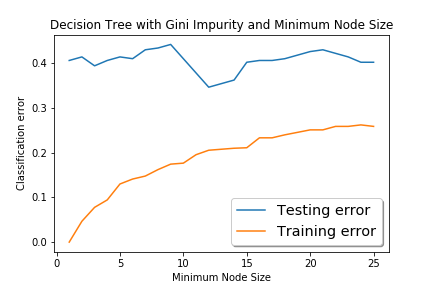
\includegraphics[scale=0.7]{2a_plot.png}
\end{figure}
\noindent
}\end{solution}
\newpage


\problem[7] Train a decision tree classifier using Gini as the impurity measure and maximal tree
depth as early stopping criterion. Try different tree depths from 2 to 20 in increments of 1. Then, on a single plot, plot both training and test classification error versus tree depth. To do this, fill in the \texttt{eval_tree_-based_model_max_depth} function in the code template for this problem.
\begin{solution}\normalfont{
\noindent
\begin{figure}[H]
\centering
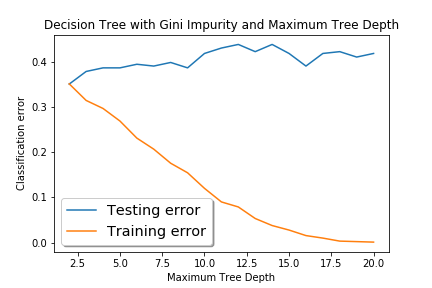
\includegraphics[scale=0.7]{2b_plot.png}
\end{figure}
\noindent
}\end{solution}
\newpage


\problem[4] For both the minimal leaf node size and maximum depth parameters tested in
the last two questions, which parameter value minimizes the test error? What effects does early stopping have on the performance of a decision tree model? Please justify your answer based on the two plots you derived.
\begin{solution}\normalfont{
For the minimal leaf node size, the test error is minimized at min\_samples\_leaf = 12. For maximum depth, the test error is minimized at max\_depth = 2. The effect that early stopping has on the performance of a decision tree model is preventing overfitting, as when the minimal leaf node size becomes too large or the maximum depth becomes too large, the decision tree has a worse test error than with respective smaller value parameters. This effect is seen in both plots in Problems 2A and 2B, as increasing the magnitude of either the minimal leaf node size or the maximum depth causes test error to increase.
}\end{solution}
\newpage


\indent\problem[2] % indent for consistency
Train a random forest classifier using Gini as the impurity measure, minimal leaf node size as early stopping criterion, and 1,000 trees in the forest. Try different node sizes from 1 to 25 in increments of 1. Then, on a single plot, plot both training and test classification error versus leaf node size.
\begin{solution}\normalfont{
\noindent
\begin{figure}[H]
\centering
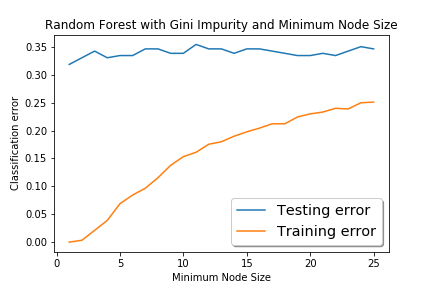
\includegraphics[scale=0.7]{2d_plot.png}
\end{figure}
\noindent
}\end{solution}
\newpage


\problem[2] Train a random forest classifier using Gini as the impurity measure, maximal tree
depth as early stopping criterion, and 1,000 trees in the forest. Try different tree depths from 2 to 20 in increments of 1. Then, on a single plot, plot both training and test classification error versus tree depth.
\begin{solution}\normalfont{
\noindent
\begin{figure}[H]
\centering
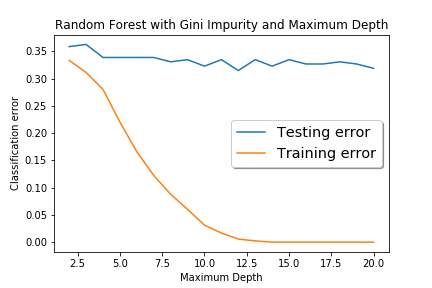
\includegraphics[scale=0.7]{2e_plot.png}
\end{figure}
\noindent
}\end{solution}
\newpage


\problem[4] For both the minimal leaf node size and maximum depth parameters tested, which
parameter value minimizes the random forest test error? What effects does early stopping have on the performance of a random forest model? Please justify your answer based on the two plots you derived.
\begin{solution}\normalfont{
For the minimal leaf node size, the test error is minimized at min\_samples\_leaf = 1. For maximum depth, the test error is minimized at max\_depth = 12. The effect that early stopping has on the performance of a random forest model is preventing slight overfitting, as the plot in Problem 2D shows that the minimum test error is for min\_samples\_leaf = 1, and the plot in Problem 2E shows that overfitting occurs past max\_depth = 12. This effect is seen in both plots in Problems 2D and 2E, as increasing the magnitude of either the minimal leaf node size or the maximum depth causes test error to increase.
}\end{solution}
\newpage


\problem[4] Do you observe any differences between the curves for the random forest and
decision tree plots? If so, explain what could account for these differences.
\begin{solution}\normalfont{
The plots of varying max\_depth for the decision tree and random forest differ, as the training error of random forest converges more quickly than the training error of decision tree does. Additionally, the test error for the max\_depth plot of decision tree is minimized at max\_depth = 1, while for random forest, max\_depth = 12 is where the minimum test error is in the plot. The differences in these plots originate from the different natures of the models used, as random forest is an ensemble model, while decision tree is only one structure.
}\end{solution}
\newpage





%%%%%%%%%%%%%%%%%%%%%%%%%%%%%%
% PROBLEM 3 
%%%%%%%%%%%%%%%%%%%%%%%%%%%%%%
\newpage
\section{The AdaBoost Algorithm [40 points]}
\materials{Lecture 6}

In this problem, you will show that the choice of the $\alpha_t$ parameter in the AdaBoost algorithm corresponds to greedily minimizing an exponential upper bound on the loss term at each iteration.

\problem[3] Let $h_t : \mathbb{R}^m \rightarrow \{-1, 1\}$ be the weak classifier obtained at step $t$, and let $\alpha_t$ be its weight. Recall that the final classifier is
\[ H(x) = \text{sign}(f(x)) = \text{sign}\bigg(\sum_{i=1}^T \alpha_t h_t(x)\bigg). \]
Suppose $\{(x_1, y_1), ..., (x_N, y_N)\} \subset \mathbb{R}^m \times \{-1, 1\}$ is our training dataset. Show that the training set error of the final classifier can be bounded from above if an an exponential loss function is used:
\[ E = \dfrac{1}{N}\sum_{i=1}^N \exp(-y_i f(x_i)) \geq \dfrac{1}{N}\sum_{i=1}^{N} \mathbbm{1}(H(x_i) \neq y_i), \]
where $\mathbbm{1}$ is the indicator function.
\begin{solution}\normalfont{
There are two cases to consider for this system for any given $(x_i, y_i)$.\\
\\
Case 1: $H(x_i) \neq y_i$.\\
\\
Since $H(x_i) \neq y_i$, by definition, $\mathbbm{1}(H(x_i) \neq y_i) = 1$. Since $H(x_i) \neq y_i$, $\text{sign}(-y_i f(x_i)) = 1$, so $\exp(-y_i f(x_i)) \geq 1$. Therefore, $\exp(-y_i f(x_i)) \geq \mathbbm{1}(H(x_i) \neq y_i)$\\
$\implies \frac{1}{N}\sum_{i=1}^N \exp(-y_i f(x_i)) \geq \frac{1}{N} \sum_{i=1}^N \mathbbm{1}(H(x_i) \neq y_i)$ for this case.\\
\\
Case 2: $H(x_i) = y_i$.\\
\\
Since $H(x_i) \neq y_i$, by definition, $\mathbbm{1}(H(x_i) \neq y_i) = 0$. For any possible $-y_i f(x_i)$, $\exp(-y_i f(x_i)) \geq 0$. Therefore, $\exp(-y_i f(x_i)) \geq \mathbbm{1}(H(x_i) \neq y_i)\implies \frac{1}{N}\sum_{i=1}^N \exp(-y_i f(x_i)) \geq \frac{1}{N} \sum_{i=1}^N \mathbbm{1}(H(x_i) \neq y_i)$ for this case.\\
\\
Since both possible cases show that $\frac{1}{N} \sum_{i=1}^N \mathbbm{1}(H(x_i) \neq y_i)$, the training set error of the final classifier can be bounded from above if an an exponential loss function is used:
\[ E = \dfrac{1}{N}\sum_{i=1}^N \exp(-y_i f(x_i)) \geq \dfrac{1}{N}\sum_{i=1}^{N} \mathbbm{1}(H(x_i) \neq y_i), \]
where $\mathbbm{1}$ is the indicator function. $\blacksquare$
}\end{solution}
\newpage


\problem[3] Find $D_{T+1}(i)$ in terms of $Z_t, \alpha_t, x_i, y_i$, and the classifier $h_t$, where $T$ is the last timestep and $t \in \{1, \dots , T\}$. Recall that $Z_t$ is the normalization factor for distribution $D_{t+1}$:
\[ Z_t = \sum_{i=1}^N D_t(i) \exp(-\alpha_t y_t h_t(x_i)). \]
\begin{solution}\normalfont{
Using the AdaBoost Weighting Update recursive forumula (lecture 6, slide 58),
\[ D_{t+1}(i) = \dfrac{D_t(i) \exp((-\alpha_t y_i h_t(x_i)))}{Z_t}, \]
where $D_1 = \frac{1}{N}$. Thus,
\[ D_2(i) = \dfrac{D_1(i)\exp{(-\alpha_1 y_i h_1(x_i))}}{Z_1}, \]
and,
\[ D_3(i) = D_2(i) \dfrac{\exp(-\alpha_2 y_i h_2(x_i))}{Z_2} = \dfrac{D_1(i)\exp(-\alpha_1 y_i h_1(x_i))}{Z_1} \dfrac{\exp(-\alpha_2 y_i h_2(x_i))}{Z_2} \]
\[= \dfrac{\frac{1}{N}\exp(-\alpha_1 y_i h_1(x_i)-\alpha_2 y_i h_2(x_i))}{Z_1 Z_2}. \]
Therefore, using the pattern that originates from the recursive formula, for $T+1$,
\[ D_{T+1}(i) = \dfrac{1}{N}\exp(-y_i \sum_{t=1}^T \alpha_t h_t(x_i)) \prod_{t=1}^T Z_t^{-1}.\;\blacksquare \]
}\end{solution}
\newpage



\problem[2] Show that $E = \sum_{i=1}^N \frac{1}{N} e^{\sum_{t=1}^T -\alpha_t y_i h_t(x_i)}$:
\begin{solution}\normalfont{
From Problem 3A, $E = \dfrac{1}{N}\sum_{i=1}^N \exp(-y_i f(x_i))$, where $f(x_i) = \sum_{t=1}^T \alpha_t h_t(x_i)$, so
\[ E = \dfrac{1}{N}\sum_{i=1}^N \exp(-y_i f(x_i)) = \sum_{i=1}^N \dfrac{1}{N} e^{-y_i f(x_i)} = \sum_{i=1}^N \dfrac{1}{N} e^{-y_i \sum_{t=1}^T \alpha_t h_t(x_i)} = \sum_{i=1}^N \dfrac{1}{N} e^{\sum_{t=1}^T -\alpha_t y_i h_t(x_i)}. \]
Therefore, $\sum_{i=1}^N \dfrac{1}{N} e^{\sum_{t=1}^T -\alpha_t y_i h_t(x_i)}$. $\blacksquare$
}\end{solution}
\newpage



\problem[5] Show that
\[ E = \prod_{t=1}^T Z_t. \]
\textit{\textbf{Hint:} Recall that $\sum_{i=1}^N D_t(i) = 1$ because D is a distribution.}
\begin{solution}\normalfont{
From Problem 3B, $D_{T+1}(i) = \dfrac{1}{N}\exp(-y_i \sum_{t=1}^T \alpha_t h_t(x_i)) \prod_{t=1}^T Z^{-1}$ Taking the sum from $\sum_{i=1}^N$ of both sides gives
\[ \sum_{i=1}^N D_{T+1}(i) = \sum_{i=1}^N \dfrac{1}{N}\exp(-y_i \sum_{t=1}^T \alpha_t h_t(x_i)) \prod_{t=1}^T Z_t^{-1} \]
\[ \implies 1 = \dfrac{1}{N} \sum_{i=1}^N \exp(-y_i \sum_{t=1}^T \alpha_t h_t(x_i)) \prod_{t=1}^T Z_t^{-1} \implies \prod_{t=1}^T Z_t = \dfrac{1}{N} \sum_{i=1}^N \exp(-y_i \sum_{t=1}^T \alpha_t h_t(x_i)) \]
\[ \prod_{t=1}^T Z_t = \dfrac{1}{N} \sum_{i=1}^N \exp(-y_i \sum_{t=1}^T \alpha_t h_t(x_i)) = \dfrac{1}{N} \sum_{i=1}^N \exp(-y_i \sum_{t=1}^T \alpha_t h_t(x_i)) \]
\[= \dfrac{1}{N} \sum_{i=1}^N \exp(-y_i f(x_i)) \implies E = \prod_{t=1}^T Z_t.\;\blacksquare \]
}\end{solution}
\newpage


\problem[5] Show that the normalizer $Z_t$ can be written as
\[ Z_t = (1 - \epsilon_t)\exp(-\alpha_t) + \epsilon_t\exp(\alpha_t) \]
where $\epsilon_t$ is the training set error of weak classifier $h_t$ for the weighted dataset:
\[ \epsilon_t = \sum_{i=1}^N D_t(i) \mathbbm{1}(h_t(x_i) \neq y_i). \]
\begin{solution}\normalfont{
From Problem 3B, $Z_t = \sum_{i=1}^N D_t(i) \exp(-\alpha_t y_t h_t(x_i))$. If $\text{sign}(y_t h_t(x_i)) = -1$,\\
then $-\alpha_t y_t h_t(x_i) = \alpha_t$. If $\text{sign}(y_t h_t(x_i)) = 1$, then $-\alpha_t y_t h_t(x_i) = -\alpha_t$. Therefore,
\[ Z_t = \sum_{i, h_t(x_i) = y_i} D_t(i) \exp(-\alpha_t) + \sum_{i, h_t(x_i) \neq y_i} D_t(i) \exp(\alpha_t) \]
\[ Z_t = \exp(-\alpha_t) \sum_{i, h_t(x_i) = y_i} D_t(i) \mathbbm{1}(h_t(x_i) \neq y_i) + \exp(\alpha_t) \sum_{i, h_t(x_i) \neq y_i} D_t(i) \mathbbm{1}(h_t(x_i) \neq y_i). \]
Since $\mathbbm{1}(h_t(x_i) \neq y_i) = 1 - \mathbbm{1}(h_t(x_i) = y_i)$,
\[ Z_t = \exp(-\alpha_t) \sum_{i, h_t(x_i) = y_i} D_t(i) (1 - \mathbbm{1}(h_t(x_i) = y_i)) + \exp(\alpha_t) \sum_{i, h_t(x_i) \neq y_i} D_t(i) \mathbbm{1}(h_t(x_i) \neq y_i) \]
\[ \implies Z_t = \exp(-\alpha_t) (1 - \epsilon_t) + \exp(\alpha_t) \epsilon_t.\;\blacksquare \]
}\end{solution}
\newpage



\problem[2] We derived all of this because it is hard to directly minimize the training set error,
but we can greedily minimize the upper bound $E$ on this error. Show that choosing $\alpha_t$ greedily to minimize $Z_t$ at each iteration leads to the choices in AdaBoost:
\[ \alpha_t^* = \dfrac{1}{2} \ln\Big(\dfrac{1-\epsilon_t}{\epsilon_t}\Big). \]
\begin{solution}\normalfont{
Minimizing $Z_t$ results in $\dfrac{\partial}{\partial \alpha} Z_t = \dfrac{\partial}{\partial \alpha}(\exp(-\alpha_t) (1 - \epsilon_t) + \exp(\alpha_t) \epsilon_t) = 0$
\[ \implies -\exp(-\alpha_t) (1 - \epsilon_t) + \exp(\alpha_t) \epsilon_t = 0 \implies \exp(\alpha_t) \epsilon_t = \exp(-\alpha_t) (1 - \epsilon_t) \]
\[\implies \ln(\exp(\alpha_t) \epsilon_t) = \ln(\exp(-\alpha_t) (1 - \epsilon_t)) \implies \ln(\exp(\alpha_t)) + \ln(\epsilon_t) = \ln(\exp(-\alpha_t)) + \ln(1 - \epsilon_t) \]
\[ \alpha_t  + \ln(\epsilon_t) = -\alpha_t + \ln(1 - \epsilon_t) \implies 2 \alpha_t = \ln(1 - \epsilon_t) - \ln(\epsilon) \implies \alpha_t^* = \dfrac{1}{2}\ln\Big(\dfrac{1 - \epsilon_t}{\epsilon_t}\Big). \]
Therefore, choosing $\alpha_t$ greedily to minimize $Z_t$ at each iteration leads to the choices in AdaBoost:
\[ \alpha_t^* = \dfrac{1}{2} \ln\Big(\dfrac{1-\epsilon_t}{\epsilon_t}\Big).\;\blacksquare\]
}\end{solution}
\newpage



\problem[14] Implement the \texttt{GradientBoosting.fit()} and \texttt{AdaBoost.fit()} methods in
the notebook provided for you. Some important notes and guidelines follow:
\begin{enumerate}[$\bullet$]
\item For both methods, make sure to work with the class attributes provided to you. Namely, after\\
\texttt{GradientBoosting.fit()} is called, \texttt{self.clfs} should be appropriately filled with the \texttt{self.n_-clfs} trained weak hypotheses. Similarly, after \texttt{AdaBoost.fit()} is called, \texttt{self.clfs} and\\
\texttt{self.coefs}
should be appropriately filled with the \texttt{self.n_clfs} trained weak hypotheses and their coefficients, respectively.
\item \texttt{AdaBoost.fit()} should additionally return an $(N, T)$ shaped numpy array D such that \texttt{D[:, t]} contains $D_{t+1}$ for each $t \in \{0, \dots, \texttt{self.n_clfs}\}$.
\item For the \texttt{AdaBoost.fit()} method, \textbf{use the 0/1} loss instead of the exponential loss.
\item The only Sklearn classes that you may use in implementing your boosting fit functions are the DecisionTreeRegressor and DecisionTreeClassifier, not GradientBoostingRegressor.
\end{enumerate}
\begin{solution}\normalfont{
}\end{solution}
\newpage


\problem[2] Describe and explain the behaviour of the loss curves for gradient boosting and for
AdaBoost. You should consider two kinds of behaviours: the smoothness of the curves and the final values that the curves approach.
\begin{solution}\normalfont{
Gradient boost had a smoother loss curve, while AdaBoost had a lower final test loss.
}\end{solution}
\newpage


\problem[2] Compare the final loss values of the two models. Which performed better on the
classification dataset?
\begin{solution}\normalfont{
AdaBoost performed better than Gradient boost, with final test losses of about 0.20 and 0.25 respectively.
}\end{solution}
\newpage


\problem[2] For AdaBoost, where are the dataset weights the largest, and where are they the
smallest?\\
\\
\textit{\textbf{Hint:} Watch how the dataset weights change across time in the animation.}
\begin{solution}\normalfont{
}\end{solution}
\newpage



\end{document}
